TODO: apraksti grafikiem un tabula līdz ko būs final version.

\section{Chatbot datu kopa}

\begin{table}[htbp]
  \centering
  \caption{Unikālo anotāciju skaits "chatbot" treniņkopā un testa kopā.}
    \begin{tabular}{lrr}
    Labels & Train & Test \\
    FindConnection & 57    & 71 \\
    DepartureTime & 43    & 35 \\
    \end{tabular}%
  \label{tab:chatbot-labels}%
\end{table}%

\begin{figure}[h] 
   \centering
   \subcaptionbox{mBERT latviešu treniņdatu kopa}{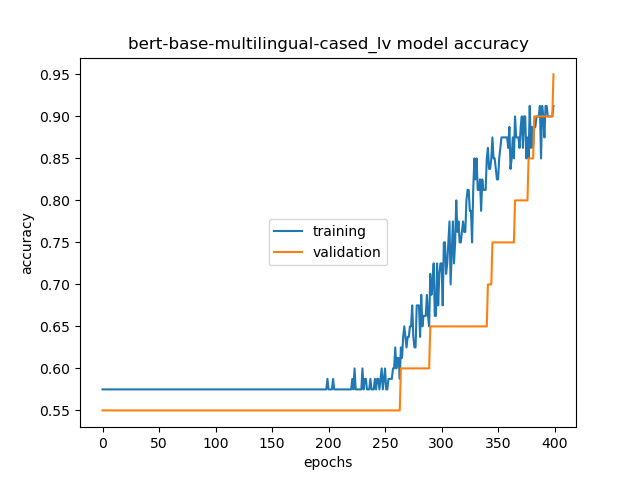
\includegraphics[width=0.49\linewidth,trim={0 0.1cm 0 0},clip]{graphs/bert-base-multilingual-cased_lv-accuracy.png}}
   \subcaptionbox{mBERT mašīntulkoto latviešu treniņdatu kopa}{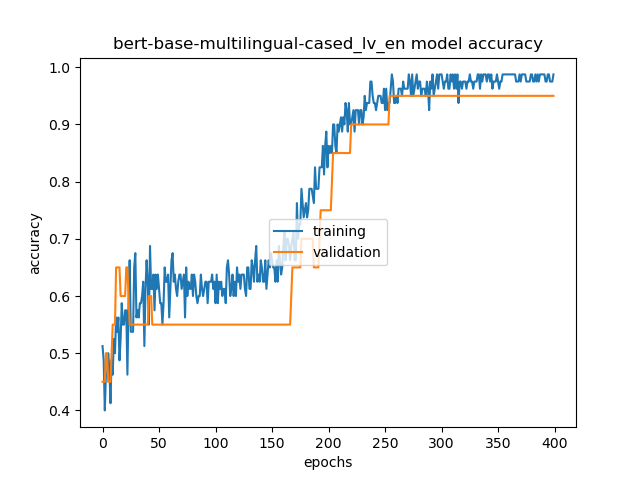
\includegraphics[width=0.49\linewidth,trim={0 0.1cm 0 0},clip]{graphs/bert-base-multilingual-cased_lv_en-accuracy.png}}
   \caption{caption} 
   \label{fig:chatbot-bert}
\end{figure}


\begin{figure}[h] 
   \centering
   \subcaptionbox{mBERT apvienotā treniņdatu kopa}{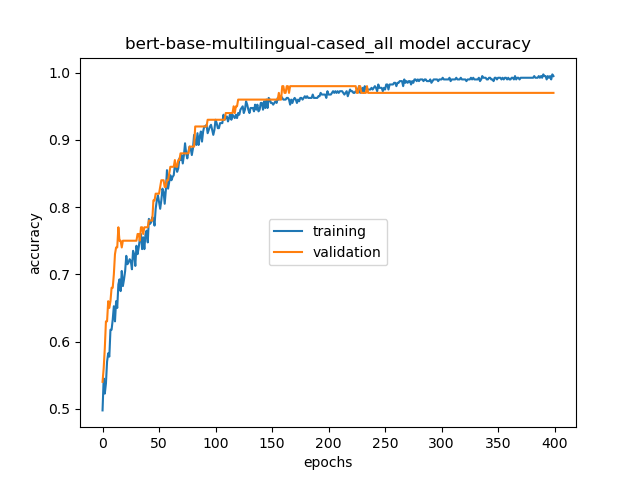
\includegraphics[width=0.49\linewidth,trim={0 0.1cm 0 0},clip]{graphs/bert-base-multilingual-cased_all-accuracy.png}}
   \subcaptionbox{mBERT apvienotā mašīntulkoto treniņdatu kopa}{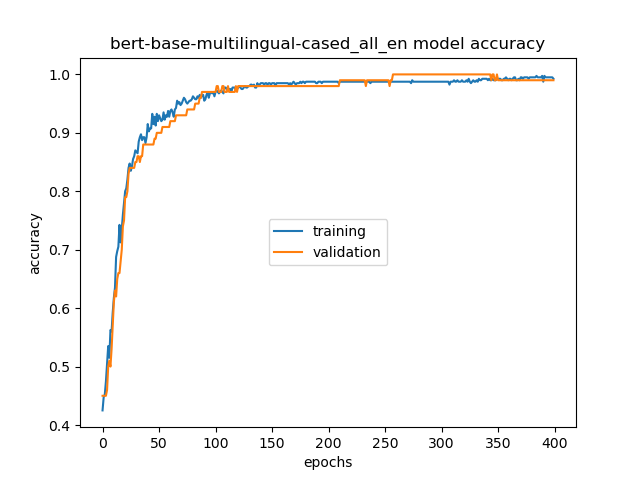
\includegraphics[width=0.49\linewidth,trim={0 0.1cm 0 0},clip]{graphs/bert-base-multilingual-cased_all_en-accuracy.png}}
   \caption{caption} 
   \label{fig:chatbot-bert-all}
\end{figure}


\begin{figure}[h] 
   \centering
   \subcaptionbox{mBERT angļu treniņdatu kopa}{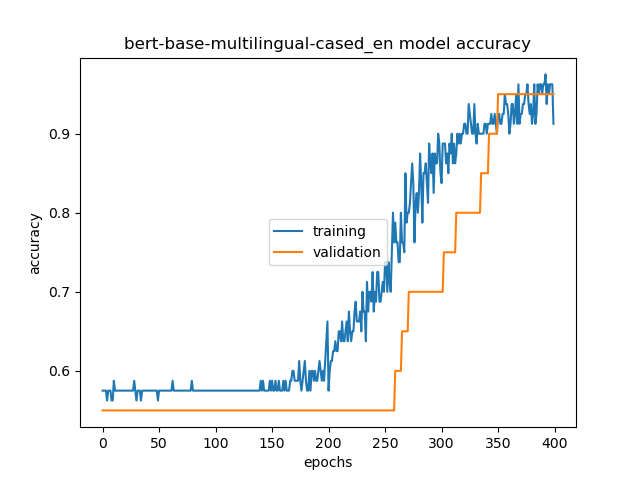
\includegraphics[width=0.49\linewidth,trim={0 0.1cm 0 0},clip]{graphs/bert-base-multilingual-cased_en-accuracy.png}}
   \subcaptionbox{XLM-RoBERTa angļu treniņdatu kopa}{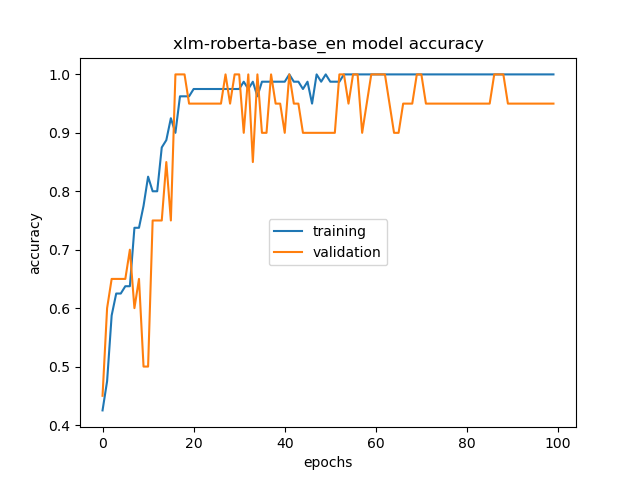
\includegraphics[width=0.49\linewidth,trim={0 0.1cm 0 0},clip]{graphs/xlm-roberta-base_en-accuracy.png}}
   \caption{caption} 
   \label{fig:chabot-bert-xlm-en}
\end{figure}


\begin{figure}[h] 
   \centering
   \subcaptionbox{XLM-RoBERTa latviešu treniņdatu kopa}{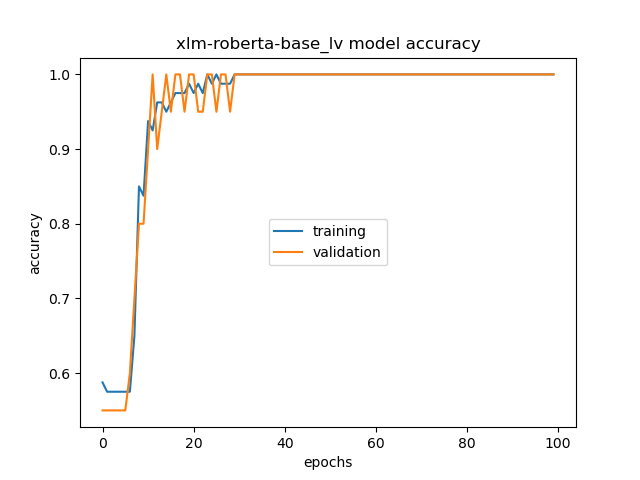
\includegraphics[width=0.49\linewidth,trim={0 0.1cm 0 0},clip]{graphs/xlm-roberta-base_lv-accuracy.png}}
   \subcaptionbox{XLM-RoBERTa mašīntulkoto latviešu treniņdatu kopa}{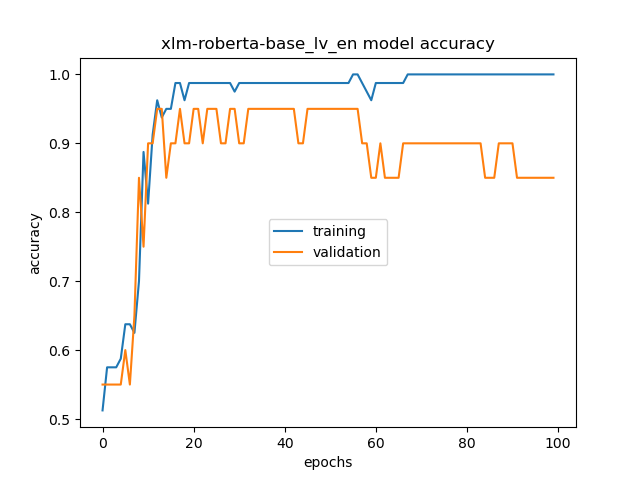
\includegraphics[width=0.49\linewidth,trim={0 0.1cm 0 0},clip]{graphs/xlm-roberta-base_lv_en-accuracy.png}}
   \caption{caption} 
   \label{fig:chatbot-xlm}
\end{figure}


\begin{figure}[h] 
   \centering
   \subcaptionbox{XLM-RoBERTa apvienotā treniņdatu kopa}{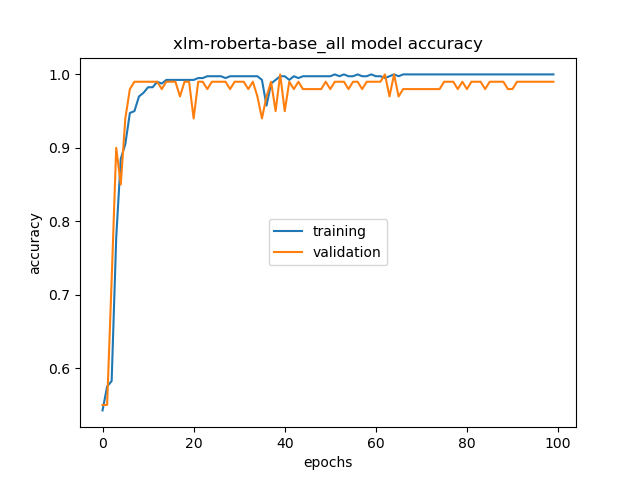
\includegraphics[width=0.49\linewidth,trim={0 0.1cm 0 0},clip]{graphs/xlm-roberta-base_all-accuracy.png}}
   \subcaptionbox{XLM-RoBERTa apvienotā mašīntulkoto treniņdatu kopa}{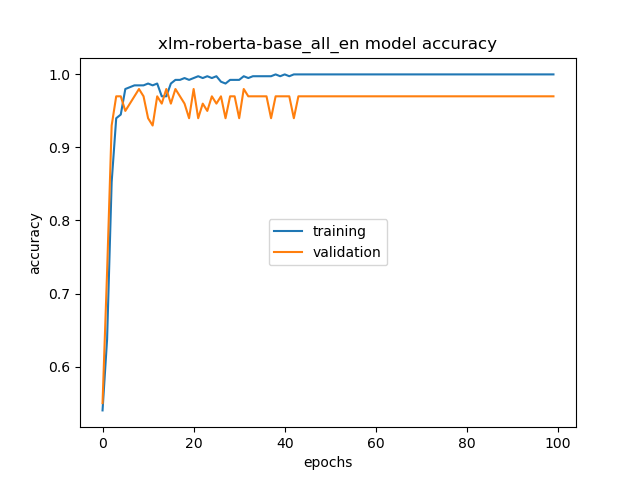
\includegraphics[width=0.49\linewidth,trim={0 0.1cm 0 0},clip]{graphs/xlm-roberta-base_all_en-accuracy.png}}
   \caption{caption} 
   \label{fig:chatbot-xlm-all}
\end{figure}


\section{Askubuntu datu kopa}


\begin{table}[htbp]
  \centering
  \caption{Unikālo anotāciju skaits "askubuntu" treniņkopā un testa kopā.}
    \begin{tabular}{lrr}
    Labels & Train & Test \\
    Software Recommendation & 17    & 40 \\
    Make Update & 10    & 37 \\
    Shutdown Computer & 13    & 14 \\
    Setup Printer & 10    & 13 \\
    None  & 3     & 5 \\
    \end{tabular}%
  \label{tab:askubuntu-labels}%
\end{table}%


\begin{figure}[h] 
   \centering
   \subcaptionbox{mBERT latviešu treniņdatu kopa}{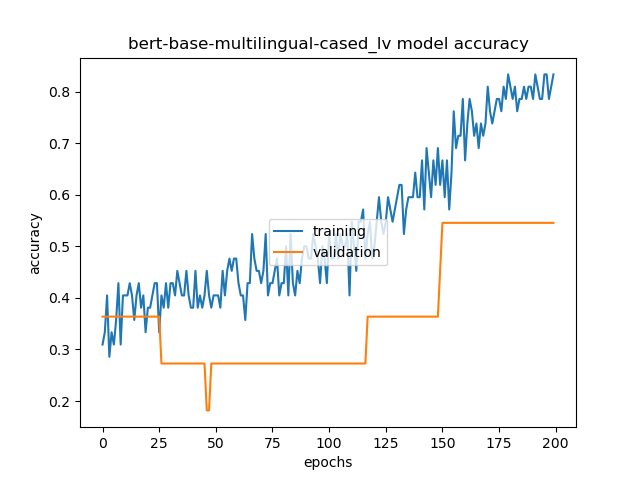
\includegraphics[width=0.49\linewidth,trim={0 0.1cm 0 0},clip]{results-3_twice-smaller-sizes/graphs/askubuntu_bert-base-multilingual-cased_lv-accuracy.png}}
   \subcaptionbox{mBERT mašīntulkoto latviešu treniņdatu kopa}{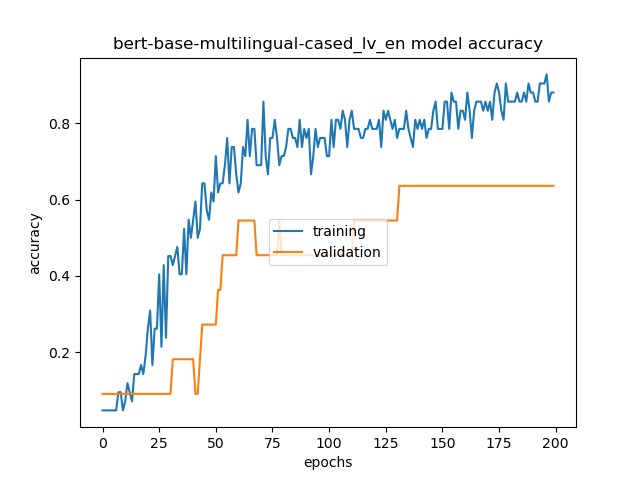
\includegraphics[width=0.49\linewidth,trim={0 0.1cm 0 0},clip]{results-3_twice-smaller-sizes/graphs/askubuntu_bert-base-multilingual-cased_lv_en-accuracy.png}}
   \caption{caption} 
   \label{fig:askubuntu-bert}
\end{figure}


\begin{figure}[h] 
   \centering
   \subcaptionbox{mBERT apvienotā treniņdatu kopa}{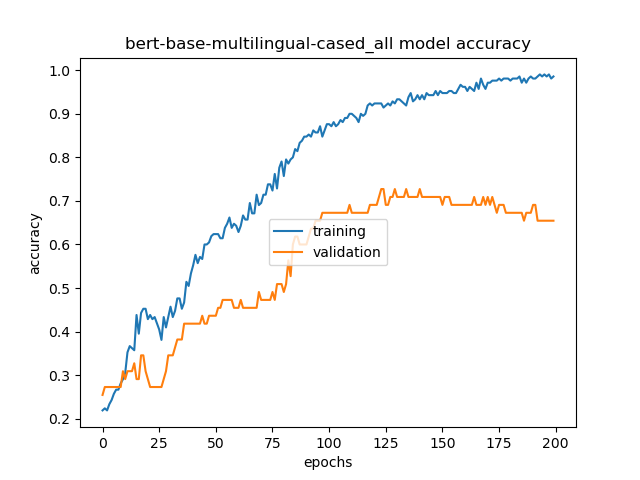
\includegraphics[width=0.49\linewidth,trim={0 0.1cm 0 0},clip]{results-3_twice-smaller-sizes/graphs/askubuntu_bert-base-multilingual-cased_all-accuracy.png}}
   \subcaptionbox{mBERT apvienotā mašīntulkoto treniņdatu kopa}{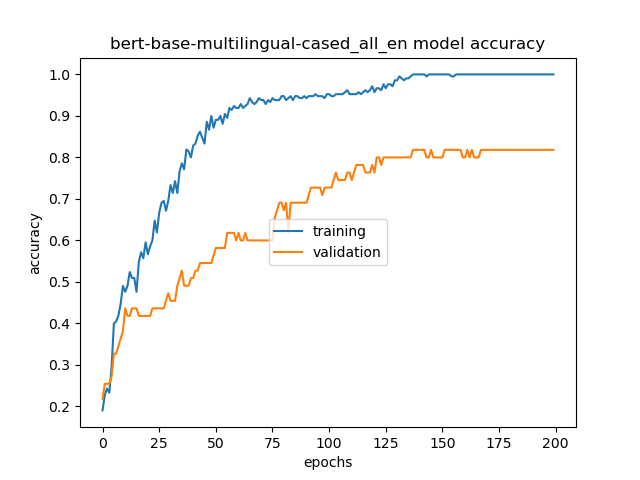
\includegraphics[width=0.49\linewidth,trim={0 0.1cm 0 0},clip]{results-3_twice-smaller-sizes/graphs/askubuntu_bert-base-multilingual-cased_all_en-accuracy.png}}
   \caption{caption} 
   \label{fig:askubuntu-bert-all}
\end{figure}


\begin{figure}[h] 
   \centering
   \subcaptionbox{mBERT angļu treniņdatu kopa}{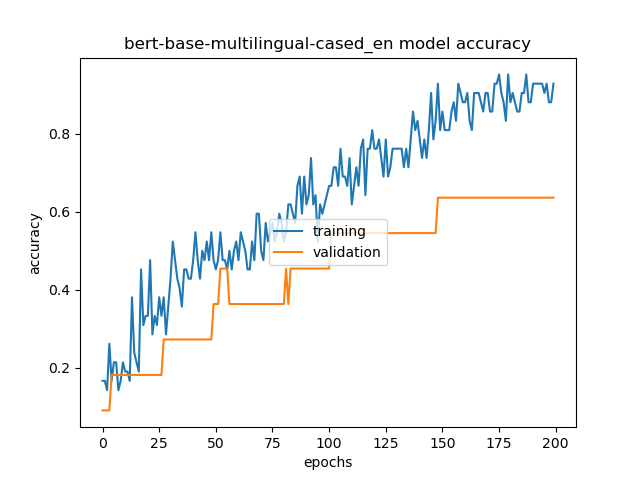
\includegraphics[width=0.49\linewidth,trim={0 0.1cm 0 0},clip]{results-3_twice-smaller-sizes/graphs/askubuntu_bert-base-multilingual-cased_en-accuracy.png}}
   \subcaptionbox{XLM-RoBERTa angļu treniņdatu kopa}{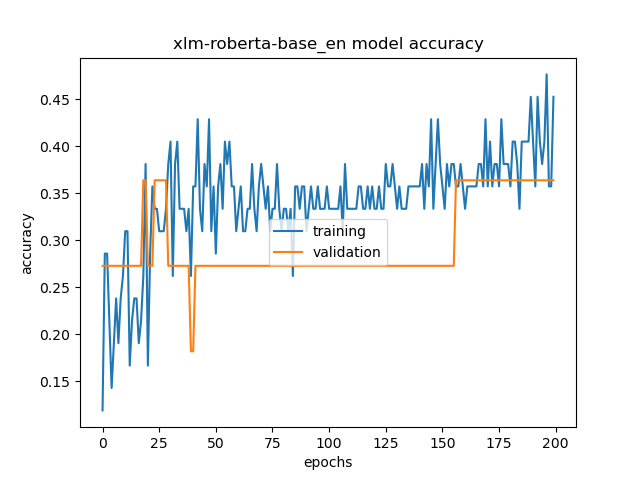
\includegraphics[width=0.49\linewidth,trim={0 0.1cm 0 0},clip]{results-3_twice-smaller-sizes/graphs/askubuntu_xlm-roberta-base_en-accuracy.png}}
   \caption{caption} 
   \label{fig:askubuntu-bert-xlm-en}
\end{figure}


\begin{figure}[h] 
   \centering
   \subcaptionbox{XLM-RoBERTa latviešu treniņdatu kopa}{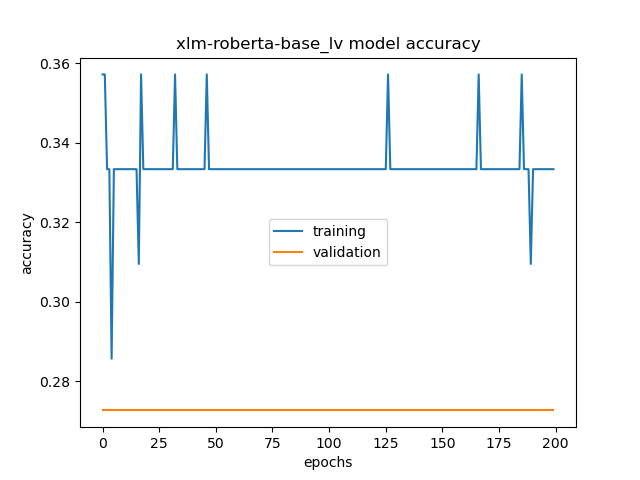
\includegraphics[width=0.49\linewidth,trim={0 0.1cm 0 0},clip]{results-3_twice-smaller-sizes/graphs/askubuntu_xlm-roberta-base_lv-accuracy.png}}
   \subcaptionbox{XLM-RoBERTa mašīntulkoto latviešu treniņdatu kopa}{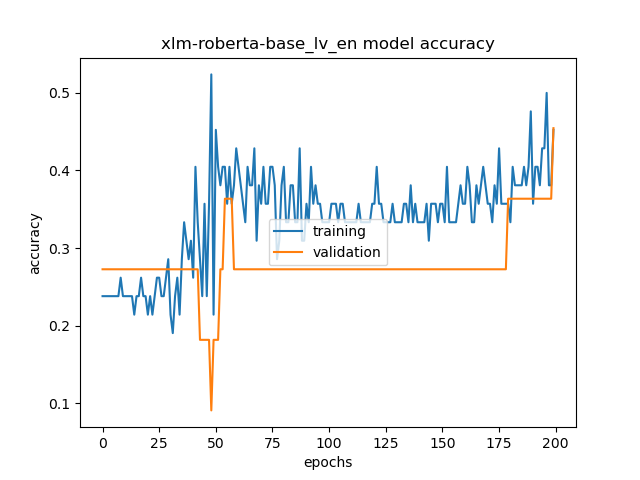
\includegraphics[width=0.49\linewidth,trim={0 0.1cm 0 0},clip]{results-3_twice-smaller-sizes/graphs/askubuntu_xlm-roberta-base_lv_en-accuracy.png}}
   \caption{caption} 
   \label{fig:askubuntu-xlm}
\end{figure}


\begin{figure}[h] 
   \centering
   \subcaptionbox{XLM-RoBERTa apvienotā treniņdatu kopa}{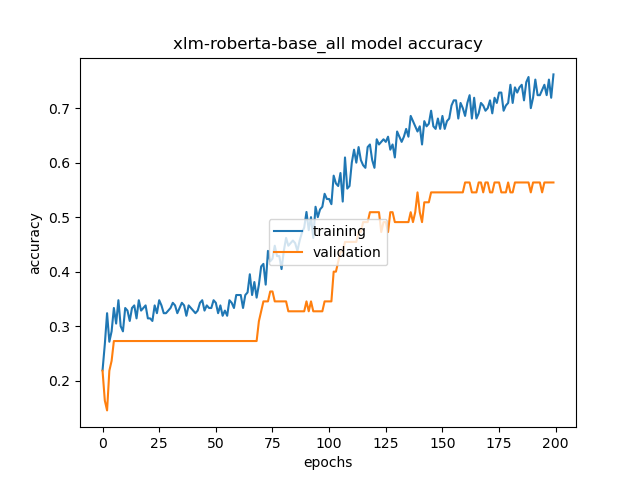
\includegraphics[width=0.49\linewidth,trim={0 0.1cm 0 0},clip]{results-3_twice-smaller-sizes/graphs/askubuntu_xlm-roberta-base_all-accuracy.png}}
   \subcaptionbox{XLM-RoBERTa apvienotā mašīntulkoto treniņdatu kopa}{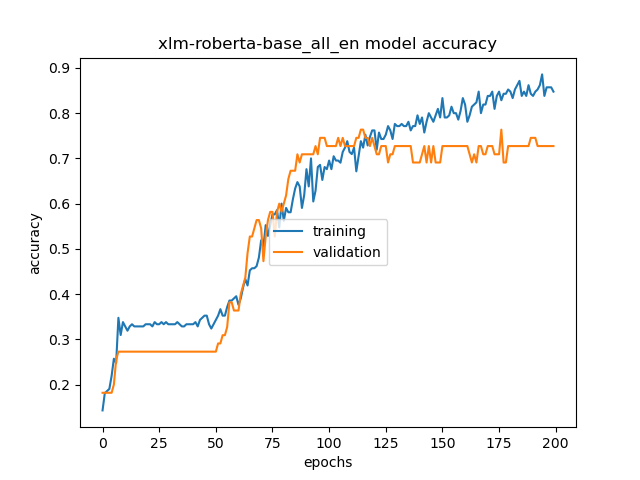
\includegraphics[width=0.49\linewidth,trim={0 0.1cm 0 0},clip]{results-3_twice-smaller-sizes/graphs/askubuntu_xlm-roberta-base_all_en-accuracy.png}}
   \caption{caption} 
   \label{fig:askubuntu-xlm-all}
\end{figure}



\section{Webapps datu kopa}


\begin{table}[htbp]
  \centering
  \caption{Unikālo anotāciju skaits "webapps" treniņkopā un testa kopā. Ar treknrakstu iezīmētas anotācijas, kuras ir pietiekami pārstāvētas, pārējās anotācijas tika apvienotas vienā jaunā anotācijā: "Other"}
    \begin{tabular}{lrr}
    Labels & Train & Test \\
    \textbf{Find Alternative} & \textbf{7} & \textbf{16} \\
    \textbf{Delete Account} & \textbf{7} & \textbf{10} \\
    \textbf{Filter Spam} & \textbf{6} & \textbf{14} \\
    \textbf{Sync Accounts} & \textbf{3} & \textbf{6} \\
    Change Password & 2     & 6 \\
    None  & 2     & 4 \\
    Export Data & 2     & 3 \\
    Download Video & 1     & 0 \\
    \end{tabular}%
  \label{tab:webapps-labels}%
\end{table}%


\begin{figure}[h] 
   \centering
   \subcaptionbox{mBERT latviešu treniņdatu kopa}{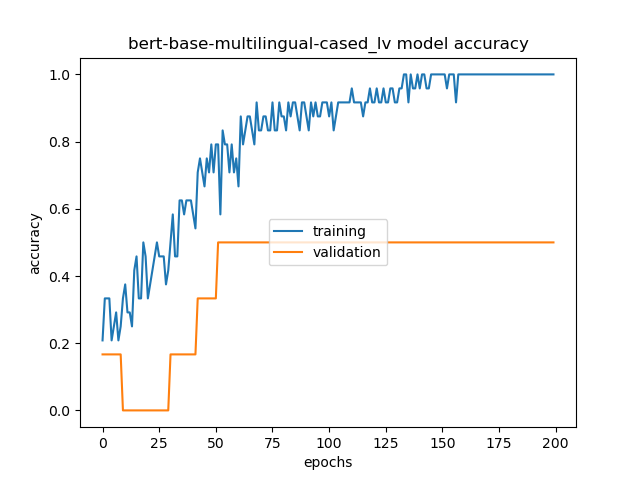
\includegraphics[width=0.49\linewidth,trim={0 0.1cm 0 0},clip]{results-5_webapps/graphs/webapps_bert-base-multilingual-cased_lv-accuracy.png}}
   \subcaptionbox{mBERT mašīntulkoto latviešu treniņdatu kopa}{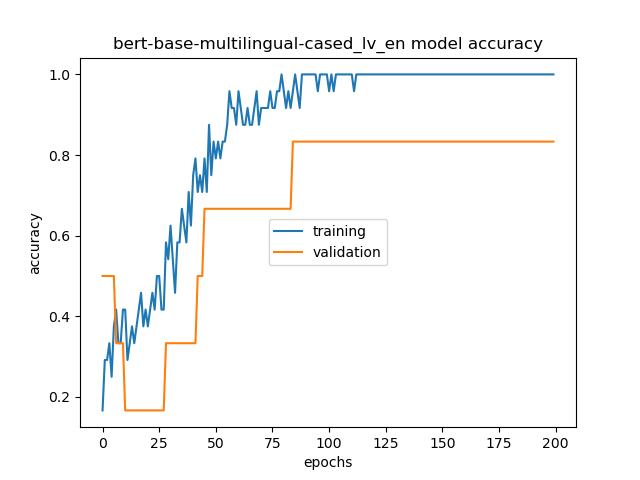
\includegraphics[width=0.49\linewidth,trim={0 0.1cm 0 0},clip]{results-5_webapps/graphs/webapps_bert-base-multilingual-cased_lv_en-accuracy.png}}
   \caption{caption} 
   \label{fig:webapps-bert}
\end{figure}


\begin{figure}[h] 
   \centering
   \subcaptionbox{mBERT apvienotā treniņdatu kopa}{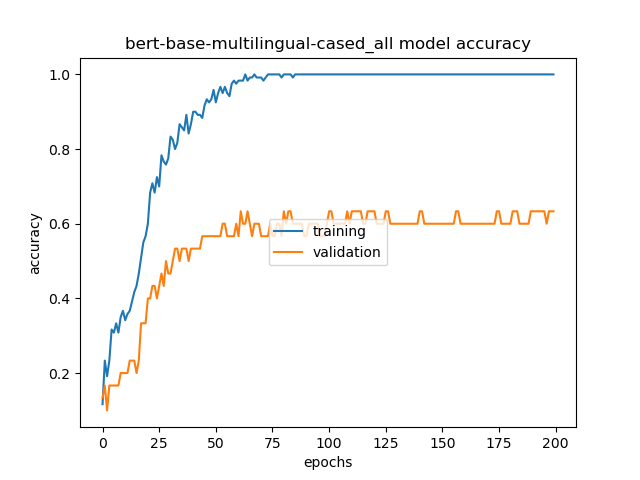
\includegraphics[width=0.49\linewidth,trim={0 0.1cm 0 0},clip]{results-5_webapps/graphs/webapps_bert-base-multilingual-cased_all-accuracy.png}}
   \subcaptionbox{mBERT apvienotā mašīntulkoto treniņdatu kopa}{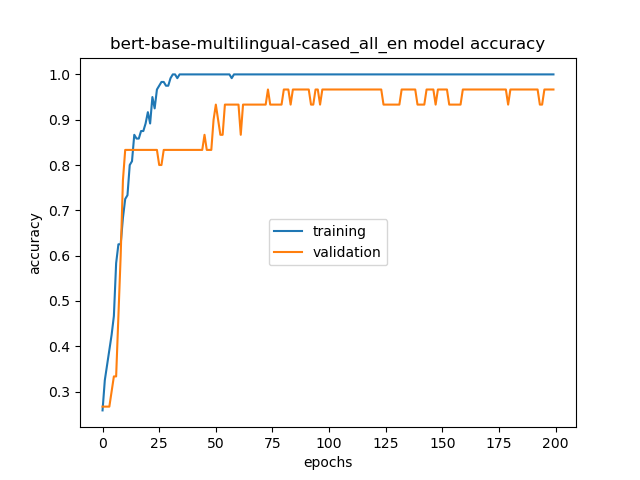
\includegraphics[width=0.49\linewidth,trim={0 0.1cm 0 0},clip]{results-5_webapps/graphs/webapps_bert-base-multilingual-cased_all_en-accuracy.png}}
   \caption{caption} 
   \label{fig:webapps-bert-all}
\end{figure}


\begin{figure}[h] 
   \centering
   \subcaptionbox{mBERT angļu treniņdatu kopa}{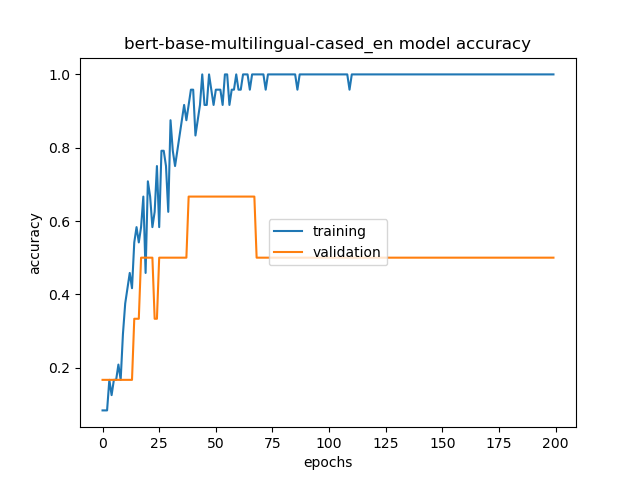
\includegraphics[width=0.49\linewidth,trim={0 0.1cm 0 0},clip]{results-5_webapps/graphs/webapps_bert-base-multilingual-cased_en-accuracy.png}}
   \subcaptionbox{XLM-RoBERTa angļu treniņdatu kopa}{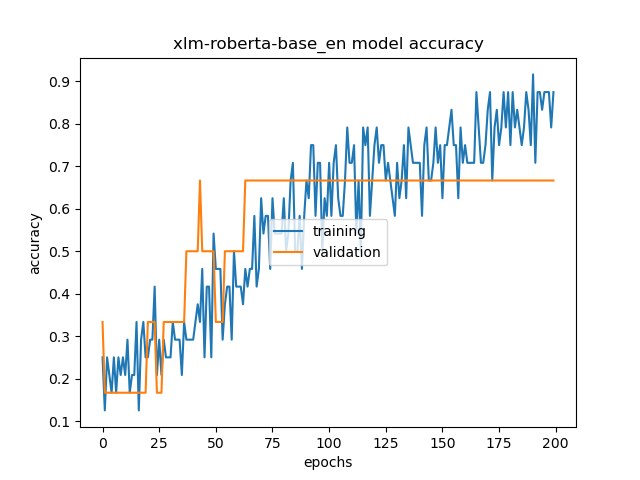
\includegraphics[width=0.49\linewidth,trim={0 0.1cm 0 0},clip]{results-5_webapps/graphs/webapps_xlm-roberta-base_en-accuracy.png}}
   \caption{caption} 
   \label{fig:webapps-bert-xlm-en}
\end{figure}


\begin{figure}[h] 
   \centering
   \subcaptionbox{XLM-RoBERTa latviešu treniņdatu kopa}{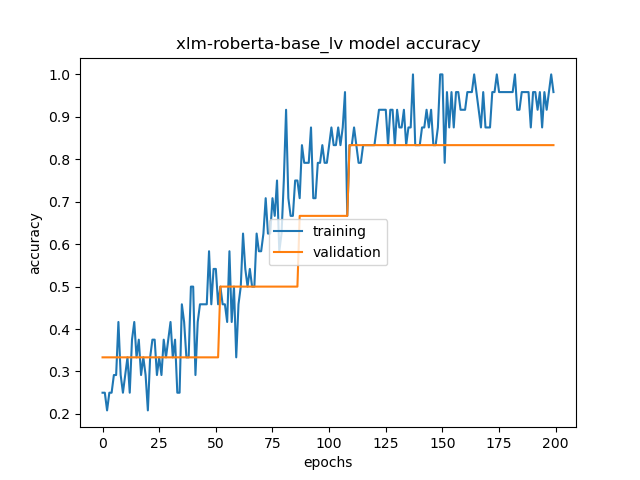
\includegraphics[width=0.49\linewidth,trim={0 0.1cm 0 0},clip]{results-5_webapps/graphs/webapps_xlm-roberta-base_lv-accuracy.png}}
   \subcaptionbox{XLM-RoBERTa mašīntulkoto latviešu treniņdatu kopa}{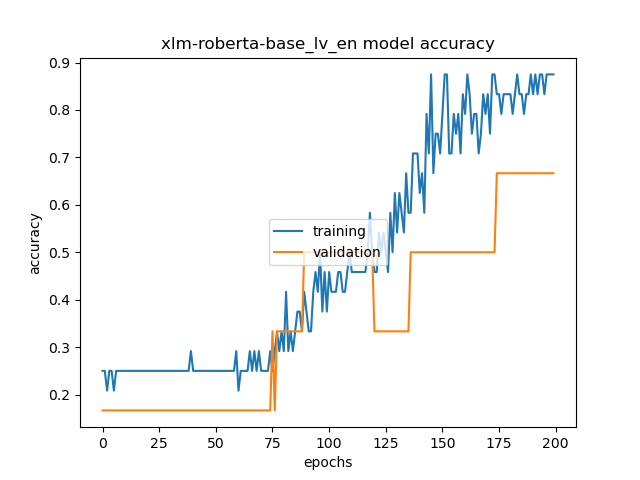
\includegraphics[width=0.49\linewidth,trim={0 0.1cm 0 0},clip]{results-5_webapps/graphs/webapps_xlm-roberta-base_lv_en-accuracy.png}}
   \caption{caption} 
   \label{fig:webapps-xlm}
\end{figure}


\begin{figure}[h] 
   \centering
   \subcaptionbox{XLM-RoBERTa apvienotā treniņdatu kopa}{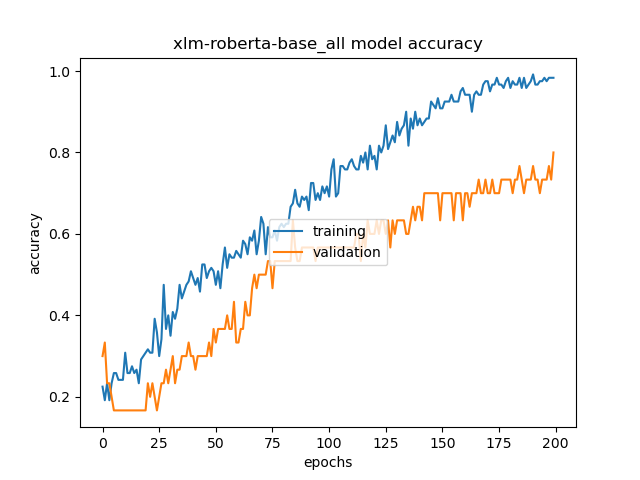
\includegraphics[width=0.49\linewidth,trim={0 0.1cm 0 0},clip]{results-5_webapps/graphs/webapps_xlm-roberta-base_all-accuracy.png}}
   \subcaptionbox{XLM-RoBERTa apvienotā mašīntulkoto treniņdatu kopa}{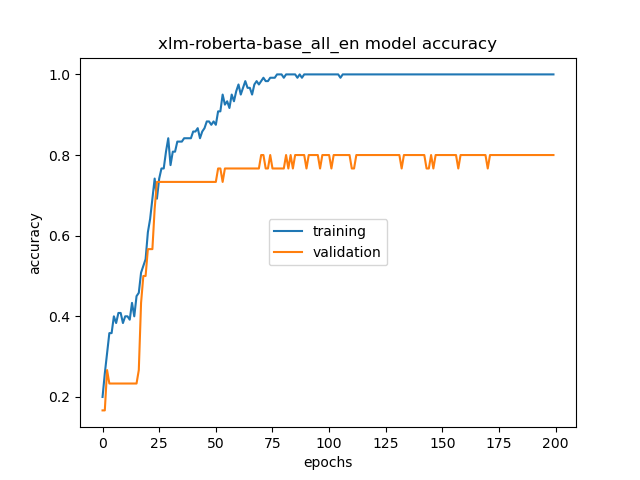
\includegraphics[width=0.49\linewidth,trim={0 0.1cm 0 0},clip]{results-5_webapps/graphs/webapps_xlm-roberta-base_all_en-accuracy.png}}
   \caption{caption} 
   \label{fig:webapps-xlm-all}
\end{figure}
